\section{Information Gathering}
Information gathering is the second phase in the iTelos methodology for knowledge graph engineering. This phase involves collecting and processing the resources needed to build the final Entity Graph (EG), following the purpose defined in the first phase. The process works with three types of datasets: data value datasets, knowledge datasets (ontologies), and language datasets. Beyond just collecting data, this phase aims to improve the quality and reusability of the gathered information through cleaning and standardization steps. This organized approach ensures the knowledge graph is built using high-quality, compatible data that effectively meets its intended purpose.

\subsection{Sources identification}
The first activity within the Information Gathering phase involves identifying and accessing relevant sources of information. This step includes examining the input sources provided and potentially exploring additional sources if the initial inputs prove insufficient.

\vspace{0.4cm}
\noindent The goal is to enable data reuse by locating pre-existing data sources that can provide the required information, by actively searching for datasets aligned with the project's objectives, ensuring the efficient use of available resources

\noindent Given the heterogeneous nature of data, multiple types of sources must be considered to effectively cover the diverse aspects of the project. To ensure high-quality and reliable information, the emphasis is placed on using "high-quality" sources, such as Pagine Gialle and catalogs of interoperable, reusable datasets. These sources are often maintained in repositories or live data catalogs (e.g., OpenData Trentino), where data and other relevant resources are published and made accessible.
\vspace{0.4cm}

\noindent\textbf{a. Data Layer\\}
\noindent The Data Layer encompasses the diverse data sources used to populate and structure information about sports facilities and events in the Trentino region. The goal is to gather comprehensive, high-quality datasets that provide detailed and relevant information. The selected sources include publicly accessible datasets and online directories, ensuring broad coverage of the various aspects related to sports and recreation. 
\vspace{0.4cm}

\noindent Below is an overview of the primary data value sources utilized in this project:
\begin{enumerate}
    \item \textbf{Overpass Turbo}
    \begin{itemize}
        \item \textit{Description}: A web-based tool for querying OpenStreetMap (OSM) data, allowing detailed searches for features like sports facilities, parks, and roads using the Overpass API. Ideal for extracting geospatial data.
        \item \textit{Access Link}: \href{https://overpass-turbo.eu/}{overpass-turbo.eu}
    \end{itemize}

    \item \textbf{OpenData Trentino}
    \begin{itemize}
        \item \textit{Description}: The official Open Data Portal of Trentino, offering access to datasets across various sectors like transportation, tourism, and public services. Supports data reuse and innovation.
        \item \textit{Access Link}: \href{https://dati.trentino.it/dataset}{dati.trentino.it}
    \end{itemize}
    
    \item \textbf{Pagine Gialle}
    \begin{itemize}
        \item \textit{Description}: An online directory of businesses in Italy, categorized by industry. Provides contact details, addresses, and user reviews for services like restaurants and sports facilities.
        \item \textit{Access Link}: \href{https://www.paginegialle.it/}{paginegialle.it}
    \end{itemize}

    \item \textbf{Festival dello Sport}
    \begin{itemize}
        \item \textit{Description}: An annual sports event in Trento featuring panels, workshops, and live sports. It gathers athletes and sports enthusiasts, providing insights into the sports industry.
        \item \textit{Access Link}: \href{https://www.ilfestivaldellosport.it/programma/}{ilfestivaldellosport.it}
    \end{itemize}

    \item \textbf{Comune di Trento}
    \begin{itemize}
        \item \textit{Description}: The official website of Trento's municipal administration, offering information on public services, events, and datasets related to urban planning and local services.
        \item \textit{Access Link}: \href{https://www.comune.trento.it/Aree-tematiche/}{www.comune.trento.it}
    \end{itemize}

    \item \textbf{List of Municipalities}
    \begin{itemize}
        \item \textit{Description}: List of municipalities of Trentino province.
        \item \textit{Access Link}: \href{https://github.com/alihamzaunitn/kdi-educationtrentino/blob/master/Datasets/Data%20Integration/Trentino%20Commune%20List.csv}{github.com/alihamzaunitn/kdi-educationtrentino}
    \end{itemize}
    
\end{enumerate}
\noindent For this project, it wasn’t possible to determine if one data source was better than another. This is because, for the type of data we handle—especially event-related data—available resources were limited. Choosing between them would have left us with very little data or, in the worst case, none at all.
\vspace{0.4cm}

\noindent\textbf{b. Knowledge Layer\\}
\noindent In designing the Knowledge Layer for Sports Facilities and Events in Trentino, we initially considered using the \textbf{General Transit Feed Specification (GTFS)}, a standard for public transit data. However, as the project's focus is not on public transit schedules or routes, the GTFS schema was deemed unsuitable. Instead, we opted to use \href{https://schema.org/docs/schemas.html}{\textbf{Schema.org}}, which better aligns with the project's requirements and is more readily available for use. 

\vspace{0.4cm}
\noindent Additionally, some property names in our model do not strictly follow the Schema.org vocabulary. This deviation was necessary to better address the specific needs and purposes of our project. This custom adaptation ensures the Knowledge Graph accurately represents the context and requirements of project's purpose.

\subsection{Datasets collection}
The Data Collection phase focuses on acquiring relevant datasets to populate the project's knowledge base. This phase involves several key steps, including the selection of data sources, gathering the data, and ensuring its quality and completeness.
\vspace{0.4cm}

\noindent The data collection process employed three main approaches:
\begin{itemize}
    \item \textbf{Direct Downloads}: Some datasets, such as those available from \textit{OpenData Trentino}, were collected directly in formats like CSV or JSON. These datasets are freely downloadable, ensuring that they are immediately usable without requiring additional extraction steps. However, it should be noted that in some circumstances, especially for \textit{OpenData Trentino}, web scraping was necessary to gather these resources more efficiently and quickly.
    \item \textbf{API}: For sources like \textit{Overpass Turbo}, an automated approach was used to gather data. The Overpass API, specifically designed for querying OpenStreetMap data, was utilized to collect information on sports facilities across the Autonomous Province of Trento. This method facilitated large-scale and precise data collection.
    \begin{lstlisting}
        [out:json][timeout:60];
        // Define the Trentino administrative area
        {{geocodeArea:Trentino}}->.searchArea;
        // Fetch data for sports centers within Trentino
        (
          nwr["leisure"~"sports_centre|pitch"](area.searchArea);
        );
        out body;
        >;
        out skel qt;
    \end{lstlisting}
    \item \textbf{Web Scraping}: In cases where structured data was not readily accessible, custom Python scripts were developed to extract information from HTML-based directories. Web scraping was used to collect data from sources such as \textit{Festival dello Sport}, \textit{Pagine Gialle}, \textit{OpenData Trentino} and \textit{Comune di Trento}. This approach allowed for the extraction of relevant data that was otherwise embedded in unstructured web pages.
\end{itemize}
\vspace{0.4cm}

\subsection{Datasets cleaning}
\noindent The primary goal of data cleaning is to eliminate noise and inconsistencies, enabling more accurate and meaningful analysis. In our case, cleaning the dataset involves addressing various issues to improve its quality. The process begins by identifying and removing duplicate entries within the dataset. Next, irrelevant data (e.g. records from years other than 2024) is filtered out to ensure the dataset remains focused and relevant to the analysis.
\vspace{0.4cm}

\noindent The data cleaning process was specifically necessary for events sourced from Trentino's open data portal. While other data sources in our project could be processed automatically, the events dataset required manual processing for two key reasons. First, as our knowledge graph focuses specifically on sports events, we needed to carefully identify and extract these from a dataset that included a wide variety of event types (cultural, social, artistic, etc.). Second, the source data structure was inconsistent, with event information spread across various fields and often embedded within long descriptive text rather than in structured fields. For instance, in the Mori dataset, the "\textit{VII\^{} Coppa Italia ParaHockey}" event had its timing information, location details, and participant categories scattered throughout a long description field, requiring careful manual extraction.


\subsection{Datasets standardization}
Standardizing a dataset involves transforming the data into a consistent format or structure. First, we ensure that all measurements use uniform units, such as converting all dates into timestamps. For our dataset, we adopted a consistent datetime format "YYYY-MM-DD HH:MM:SS" (e.g., "2024-02-10 20:30:00"), with events missing specific time information defaulting to "00:00:00". Next, we focus on maintaining consistent naming conventions, making sure terms and locations are written uniformly (e.g., "Trento" vs. "Trento city"), and standardizing categorical data to follow a consistent format (e.g., using "True" and "False" instead of "Yes" and "No"). This process is very important in our case, as it facilitates the seamless integration of data from multiple sources into a cohesive dataset.
\vspace{0.4cm}

\noindent\textbf{a. Data Layer\\}
For the data layer part, we performed a cross-check among the different cleaned datasets to ensure consistency, particularly for attributes that reference IDs from other datasets. For instance, in the \textit{Sport Facility} dataset, attributes like "\textit{sports}" and "\textit{location}" reference the IDs from the Sport and Location datasets, respectively. This ensures that the data is interconnected, allowing accurate representation of which sports are available at a given facility and its geographical context. By validating these cross-references, we establish a coherent data structure.

\vspace{0.4cm}

\noindent\textbf{b. Knowledge Layer\\}
After data acquisition and pre-processing to ensure quality and consistency, the tables below presents the final structure of our datasets for sports facilities and their associated events.

\textbf{\normalsize I. Sport}
\vspace{-7pt}
\begin{table}[H]
    \centering
    \begin{tabular}{|c|c|c|}
        \hline
        \textbf{CSV File} & \textbf{Columns} \\ \hline
        Sport & id, name \\ \hline
        Sport Facility & id, legalName, openingHours, telephone, email, url, sports, location \\ \hline
        PadelCourt & id, name, covered \\ \hline
        TennisCourt & id, name, surface, lit, covered \\ \hline
        VolleyballField & id, name, surface, lit \\ \hline
    \end{tabular}
\end{table}

\textbf{\normalsize II. Events}
\vspace{-7pt}
\begin{table}[H]
    \centering
    \begin{tabular}{|c|c|c|}
        \hline
        \textbf{CSV File} & \textbf{Columns} \\ \hline
        Event & id, name, startDate, endDate, sports, location, organization, guests \\ \hline
        Guest & id, givenName, familyName \\ \hline
        Organization & id, name \\ \hline
    \end{tabular}
\end{table}

\textbf{\normalsize III. Location}
\vspace{-7pt}
\begin{table}[H]
    \centering
    \begin{tabular}{|c|c|c|}
        \hline
        \textbf{CSV File} & \textbf{Columns} \\ \hline
        Location & id, address, municipality \\ \hline
    \end{tabular}
\end{table}

\textbf{\normalsize IV. End User}
\vspace{-7pt}
\begin{table}[H]
    \centering
    \begin{tabular}{|c|c|c|}
        \hline
        \textbf{CSV File} & \textbf{Columns} \\ \hline
        EndUser & id, givenName, familyName, birthDate, hasOccupation \\ \hline
    \end{tabular}
\end{table}

\subsection{Data cleaning and standardization explanation}
In this section, we provide a detailed explanation, accompanied by snapshots, of the steps we took to transform the raw dataset into a cleaned and subsequently standardized dataset for our project. We began with a collection of unstructured and inconsistent event data, encountering common issues such as missing fields, duplicate entries, and non-uniform formatting. Specifically, when working with data obtained from OpenData Trentino, we faced additional challenges: the datasets often had different structures and included an extensive number of attributes per event (in some cases, more than 40 fields).
\vspace{0.4cm}

\noindent As shown in Figure \ref{fig:raw_data}, many of these attributes were not relevant to our project goals, containing extraneous or redundant information that needed to be filtered out. Our process involved identifying and selecting only the most pertinent fields to ensure a streamlined and standardized dataset ready for integration into the knowledge graph.
\begin{figure}[H]
    \centering
    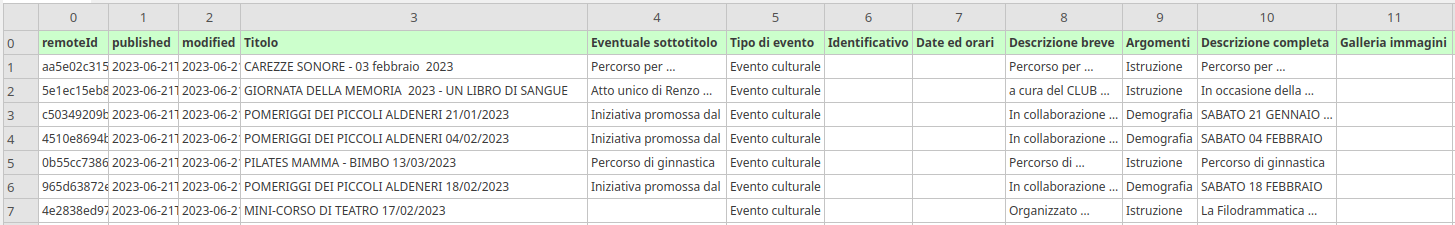
\includegraphics[width=1\linewidth]{knowdive-files/raw_dataset.png}
    \caption{Raw dataset format}
    \label{fig:raw_data}
\end{figure}

\noindent Then, during the cleaning process, we resolved inconsistencies by removing duplicate entries and correcting formatting issues. Specifically, we eliminated numerous irrelevant attributes from the raw data, such as \textit{"published"} and \textit{"modified"}, as they were not essential for our project objectives. Additionally, we extracted useful information (such as dates, times, and locations) from the \textit{"descrizione completa"} field, where this data was often embedded. As shown in Figure \ref{fig:cleaned_data}, this meticulous cleaning process allowed us to reduce noise and significantly improve the overall quality and relevance of the dataset.
\begin{figure}[H]
    \centering
    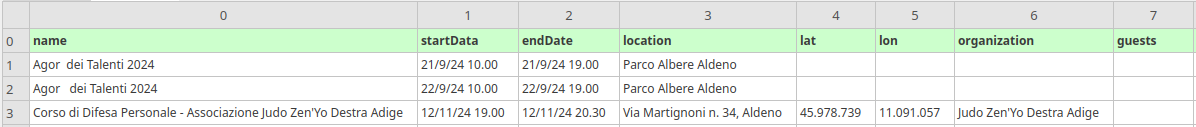
\includegraphics[width=1\linewidth]{knowdive-files/cleaned_dataset.png}
    \caption{Dataset after cleaning process}
    \label{fig:cleaned_data}
\end{figure}

\noindent Finally, we standardized the dataset to ensure consistency and compatibility with our project requirements. This involved restructuring key fields such as event names, dates, and locations to adhere to a uniform format. For instance, we standardized date entries to the format "YYYY-MM-DD HH:MM:SS" and ensured that all textual information was consistent in structure and style. 
\vspace{0.4cm}

\noindent Additionally, we conducted a "dataset integration" phase, where we linked related datasets to create meaningful connections. For example, we connected the Guest CSV with the Event CSV by associating the \textit{id} of each guest with the corresponding event instance. This step allowed us to establish relationships between datasets, enriching the overall data structure and improving its utility for our knowledge graph. As shown in Figure \ref{fig:standardized_data}, the event \textit{"ALESSANDRO COLOMBO: TAGLIATO PER VIVERE"} has the guest number \textit{8} which corresponds to \textit{"Alessandro Colombo"} in the Guest CSV in Figure \ref{fig:guest_csv} .

\begin{figure}[H]
    \centering
    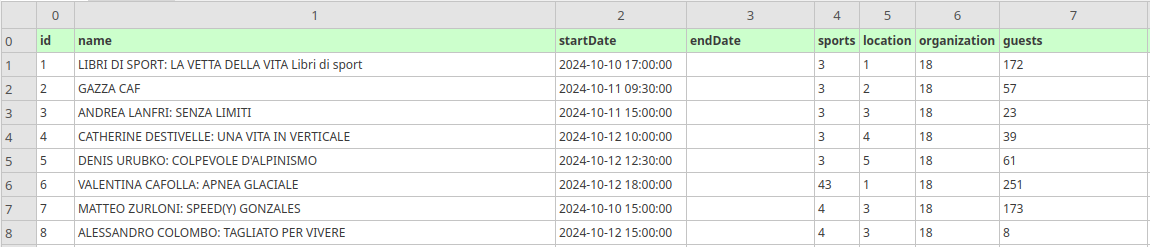
\includegraphics[width=1\linewidth]{knowdive-files/standardized_dataset.png}
    \caption{Dataset after standardization process}
    \label{fig:standardized_data}
\end{figure}
\begin{figure}
    \centering
    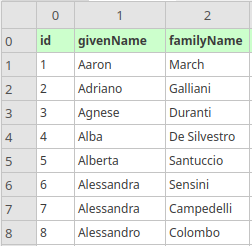
\includegraphics[width=0.23\linewidth]{knowdive-files/guest_dataset.png}
    \caption{Guest CSV}
    \label{fig:guest_csv}
\end{figure}

%-------------------------------------------------------------------------------------
\mycomment{
    In this section the second main input for the project is described, namely the data source list (if available). The resources (language, schema and data values) available as input for projects, has to be properly described. More in details for each resource has to be reported:
    \begin{itemize}
        \item The name, and the description of the information the resource is carrying.
        \item Type of resource. If it is a language, schema or data value dataset.
        \item The source from which such resource can be collected.
        \item If the resources is diversity-aware (thus already produced by iTelos) or needs to be improved in terms of diversity (i.e., data coming from low quality sources). 
    \end{itemize}
    
    Moreover, this section aims at reporting the execution of the activities involved in the Information Gathering iTelos phase.\\
    
    \noindent Information Gathering sub activities:
    \begin{itemize}
            \item Sources identification
            \item Datasets collection
            \item Datasets cleaning
            \item Datasets standardization
    \end{itemize}
    
    
    \noindent The report of the work done during the first phase of the methodology, has to includes also the description of the different choices made, with their strong and weak points. In other words the report should provide to the reader, a clear description of the reasoning conducted by all the different team members.
}